
\chapter[Decision trees (2 of 2)]{\huge\selectfont{Decision
trees for classification (2 of 2)}}
\label{ch:decisionTrees2}

\smallskip
\section{Decision Trees in Python}

\index{nested if statements@nested \texttt{if} statements}
\index{indentation}

Our decision tree pictures from chapter~\ref{ch:decisionTrees1} were quite
illustrative, but of course to actually automate something, we have to write
code rather than draw pictures. What would Figure~\ref{fig:decisionTree}
(p.~\pageref{fig:decisionTree}) look like in Python code? It's actually pretty
simple, although there's a lot of nested indentation. See if you can follow the
flow in Figure~\ref{fig:pythonDT}.

\begin{figure}[h]
\centering
\begin{Verbatim}[fontsize=\footnotesize,samepage=true,frame=single,framesep=3mm,xleftmargin=1cm,xrightmargin=1cm]
def predict(major, age, gender):
    if major == 'PSYC':
        return 'No'
    elif major == 'MATH':
        if gender == 'M':
            return 'No'
        elif gender == 'F' or gender == 'O':
            return 'Yes'
    elif major == 'CPSC':
        if age == 'young':
            return 'Yes'
        elif age == 'middle':
            return 'No'
        elif age == 'old':
            if gender == 'M' or gender == 'O':
                return 'Yes'
            elif gender == 'F':
                return 'No'
\end{Verbatim}
\caption{A Python implementation of the decision tree in
Figure~\ref{fig:decisionTree}.}
\label{fig:pythonDT}
\end{figure}

\index{predict@\texttt{predict()}}

Here we're defining a function called \texttt{predict()} that takes three
arguments, one for each feature value. The eye-popping set of
\texttt{if}/\texttt{elif}/\texttt{else} statements looks daunting at first, but
when you scrutinize it you'll realize it perfectly reflects the structure of
the purple diagram. Each time we go down one level of the tree, we indent one
tab to the right. The body of the ``\texttt{if major == \textquotesingle
PSYC\textquotesingle :}'' statement is very short because the left-most branch
of the tree (for Psychology) is very simple. The ``\texttt{elif major ==
\textquotesingle CPSC\textquotesingle :}'' body, by contrast, has lots of
nested internal structure precisely because the right-most branch of the tree
(for Computer Science) is complex. \textit{Etc.}

\begin{samepage}
If we call this function, it will give us exactly the same predictions we
calculated by hand on p.~\pageref{decisionTreeExamples}:

\begin{Verbatim}[fontsize=\footnotesize,samepage=true,frame=single,framesep=3mm]
print(predict('PSYC','M','old'))
print(predict('MATH','O','young'))
print(predict('CPSC','F','old'))
\end{Verbatim}
\vspace{-.2in}

\begin{Verbatim}[fontsize=\footnotesize,samepage=true,frame=leftline,framesep=5mm,framerule=1mm]
No
Yes
No
\end{Verbatim}
\end{samepage}

\section{Decision Tree induction}

Okay, so now we understand what a decision tree is, and even how to code one up
in Python. The key question that remains is: how do we figure out what tree to
build?

There are lots of different choices, even for our little videogame example. We
could put any of the three features at the root. For each branch from the root,
we could put either of the other features, or we could stop with a leaf. And
the leaf could be a \texttt{Yes} leaf or a \texttt{No} leaf. That's a lot of
``coulds.'' How can we know what a \textit{good} tree might be --
\textit{i.e.}, a tree that classifies new points more or less correctly?

\index{training data}
\index{inductive reasoning}

The answer, of course, is to take advantage of the training data. It consists
of labeled examples that are supposed to be our guide. Using the training data
to ``learn'' a good tree is called \textbf{inducing} a decision tree. Let's see
how.

\subsection{``Greedy'' algorithms}

\index{greedy (algorithm)}

Our decision tree induction algorithm is going to be a \textbf{greedy} one.
This means that instead of looking ahead and strategizing about future nodes
far down on the tree, we're just going to grab the immediate best-looking
feature at every individual step and use that. This won't by any means
guarantee us the best possible tree, but it will be quick to learn one.

\index{chess}

An illustration to help you understand greedy algorithms is to think about a
strategy game like chess. If you've ever played chess, you know that the only
way to play well is to think ahead several moves, and anticipate your
opponent's probable responses. You can't just look at the board na\"{i}vely and
say, ``why look at that: if I move my rook up four squares, I'll capture my
opponent's pawn! Let's do it!'' Without considering the broader implications of
your move, you're likely to discover that as soon as you take her pawn, she
turns around and takes your rook because she's lured you into a trap.

A \textit{greedy} algorithm for chess would do exactly that, however. It would
just grab whatever morsel was in front of it without considering the fuller
consequences. That may seem really dumb -- and it is, for chess -- but for
certain other problems it turns out to be a decent approach. And decision tree
induction is one of those.

The reason we resort to a greedy algorithm is that for any real-sized data set,
\textit{the number of possible trees to consider is absolutely overwhelming.}
There's simply not enough time left in the universe to look at them all -- and
that's not an exaggeration. So you have to find \textit{some} way of picking a
tree without actually contemplating every one, and it turns out that grabbing
the immediately best-looking feature at each level is a pretty good way to do
that.

\subsection{Choosing ``the immediate best'' feature}

Now what does that mean, anyway: ``choosing the immediate best feature?'' We're
going to define it as follows: the best feature to put at any given node is
\textit{the one which, if we did no further branching from that node but
instead put only leaves below it, would classify the most training points
correctly.} Let's see how this works for the videogame example.

\index{value\_counts@\texttt{.value\_counts()} method (Pandas)}
\index{groupby@\texttt{.groupby()} method (Pandas)}

Our left-most feature in the \texttt{DataFrame} is \textsf{Major}, so let's
consider that one first. Suppose we put \textsf{Major} at the root of the tree,
and then made each of its branches lead to leaves. What value should we predict
for each of the majors? Well, we can answer that with another clever use of
\texttt{.value\_counts()}, this time conjoining it with a call to
\texttt{.groupby()}. Check out this primo line of code:

\begin{Verbatim}[fontsize=\small,samepage=true,frame=single,framesep=3mm]
students.groupby('Major').VG.value_counts()
\end{Verbatim}

Stare hard at that code. You'll realize that all these pieces are things you
already know: we're just combining them in new ways. That line of code says
``take the entire \texttt{students} \texttt{DataFrame}, but treat each of the
majors as a separate group. And what should we do with each group? Well, we
count up the values of the \texttt{VG} column for the rows in that group.'' The
result is as follows:

\begin{Verbatim}[fontsize=\small,samepage=true,frame=leftline,framesep=5mm,framerule=1mm]
Major  VG 
PSYC   No     3
       Yes    2
MATH   No     3
       Yes    1
CPSC   No     4
       Yes    4
Name: VG, dtype: int64
\end{Verbatim}

We can answer ``how many would we get right?'' by reading right off that chart.
For the \texttt{PSYC} majors, there are two who play videogames and three who
do not. Clearly, then, if we presented a Psychology major to this decision
tree, it ought to predict '\texttt{No}', and that prediction would be correct
for 3 out of the 5 Psychology majors on record. For the \texttt{MATH} majors,
we would again predict '\texttt{No}', and we'd be correct 3 out of \textit{4}
times. Finally, for the \texttt{CPSC} majors, we have 4 \texttt{Yes}es and 4
\texttt{No}s, so that's not much help. We essentially have to pick randomly
since the training data doesn't guide us to one answer or the other. Let's
choose `\texttt{Yes}' for our Computer Science answer, just so it's different
than the others. The best one-level decision tree that would result from
putting \textsf{Major} at the top is therefore depicted in
Figure~\ref{fig:majorOnTop}. It gets \textbf{ten} out of the seventeen training
points correct (59\%). Your reaction is probably ``Big whoop -- we got that
good a score just using the prior, and ignoring all the features!'' Truth.
Don't lose hope, though: \textsf{Major} was only one of our three choices.

\begin{figure}[ht]
\centering
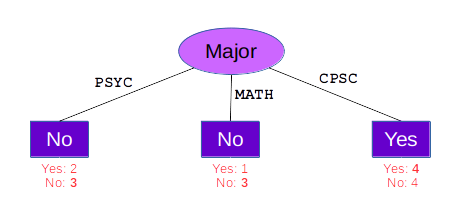
\includegraphics[width=0.9\textwidth]{majorOnTop.png}
\caption{A one-level decision tree if we put the \textsf{Major} feature at the
root -- it would classify \textbf{ten} of the seventeen training points
correctly.}
\label{fig:majorOnTop}
\end{figure}

Let's repeat this analysis for the other two features and see if either one
fares any better. Here's the query for \textsf{Age}:

\begin{Verbatim}[fontsize=\small,samepage=true,frame=single,framesep=3mm]
students.groupby('Age').VG.value_counts()
\end{Verbatim}

This yields:

\begin{Verbatim}[fontsize=\small,samepage=true,frame=leftline,framesep=5mm,framerule=1mm]
Age     VG 
middle  No     6
        Yes    2
old     Yes    2
        No     1
young   No     3
        Yes    3
Name: VG, dtype: int64
\end{Verbatim}

Making the sensible predictions at the leaves based on these values gives the
tree in Figure~\ref{fig:ageOnTop}. It gets \textbf{eleven} points right (65\%)
-- a bit of an improvement.

\begin{figure}[ht]
\centering
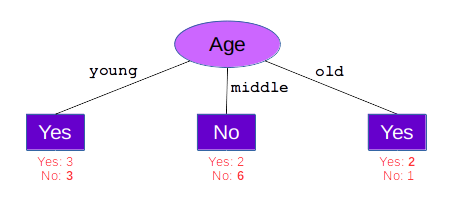
\includegraphics[width=0.8\textwidth]{ageOnTop.png}
\caption{A one-level decision tree if we chose the \textsf{Age} feature for the
root -- it would classify \textbf{eleven} of the seventeen training points
correctly.}
\label{fig:ageOnTop}
\end{figure}

Finally, we could put \textsf{Gender} at the root. Here's the query for it:

\begin{samepage}
\begin{Verbatim}[fontsize=\small,samepage=true,frame=single,framesep=3mm]
students.groupby('Gender').VG.value_counts()
\end{Verbatim}
\vspace{-.2in}

\begin{Verbatim}[fontsize=\small,samepage=true,frame=leftline,framesep=5mm,framerule=1mm]
Gender  VG 
F       No     8
        Yes    2
M       Yes    5
        No     1
O       No     1
Name: VG, dtype: int64
\end{Verbatim}
\end{samepage}

Paydirt! Splitting on the \textsf{Gender} feature first, as shown in
Figure~\ref{fig:genderOnTop}, gets us a whopping \textbf{fourteen} points
correct, or over 82\%. This is clearly the winner of the three. And since we're
being greedy and not bothering to look further downstream anyway, we hereby
elect to put \textsf{Gender} at the root of our tree.

\begin{figure}[ht]
\centering
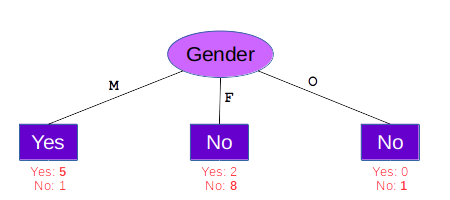
\includegraphics[width=0.8\textwidth]{genderOnTop.png}
\caption{A one-level decision tree if we chose the \textsf{Gender} feature for
the root. It would classify \textbf{fourteen} of the seventeen training points
correctly -- easily the best of the three choices.}
\label{fig:genderOnTop}
\end{figure}

It's worth taking a moment to look at those \texttt{.value\_counts()} outputs
and see if you can develop some intuition about why \textsf{Gender} worked so
much better at the root than the other two features did. The reason is that for
this data set, \textsf{Gender} split the data into groups that were more
\textbf{homogeneous} than the other splits gave. ``Homogeneous'' here means
that each group was more ``pure,'' or put another way, more lopsided towards
one of the labels. \textsf{Gender} gave us a 5-to-1 lopsided ratio on the
\texttt{M} branch, and an even more lopsided 2-to-8 ratio on the \texttt{F}
branch. Intuitively, this means that \textsf{Gender} really is correlated with
videogame use, and this shows up in purer splits. Contrast this with the
situation when we split on \textsf{Major} first, and we ended up with a yucky
4-to-4 ratio on the \texttt{CPSC} branch. An even split is the worst of all
possible worlds: here, it means that learning someone's a Computer Science
major doesn't tell you jack about their videogame use. That in turn means it's
pretty useless to split on.

\subsection{Lather, rinse, repeat}

\index{turtle}

So far, we've done all that work just to figure out which feature to put at the
root of our tree. Now, we progress down each of the branches and do the exact
same thing: figure out what to put at each branch. We'll continue on and on
like this for the entire tree. It's turtles all the way down.

% To keep this chapter at least somewhat brief, we'll do just one more layer of
% the tree.

Let's consider the \textit{left} branch of Figure~\ref{fig:genderOnTop}. What
do we do with males? There are now only two remaining features to split on. (It
wouldn't make sense to split on \textsf{Gender} again, since the only people
who will reach the left branch are males anyway: there'd be nothing to split
on.)

Thus we could put either \textsf{Major} or \textsf{Age} at that left branch. To
figure out which one is better, we'll do the same thing we did before, only
with one slight change: now, we need to consider \textit{only males} in our
analysis.

We augment our primo line of code from above with a query at the beginning, so
that our counts include only males:

\begin{Verbatim}[fontsize=\footnotesize,samepage=true,frame=single,framesep=3mm]
students[students.Gender=="M"].groupby('Major').VG.value_counts()
\end{Verbatim}
\vspace{-.2in}

\begin{Verbatim}[fontsize=\small,samepage=true,frame=leftline,framesep=5mm,framerule=1mm]
Major  VG 
CPSC   Yes    3
MATH   No     1
       Yes    1
PSYC   Yes    1
Name: VG, dtype: int64
\end{Verbatim}

Wow, cool: the \texttt{CPSC} and \texttt{PSYC} folks are perfectly homogeneous
now. If we end up deciding to split on \textsf{Major} here, we can put
permanent dark purple squares for each of those majors simply declaring
``Yes.'' In all, splitting here gives us 5 out of 6 correct. The
tree-in-progress we'd end up with is in Figure~\ref{fig:maleMajorSplit}.

\begin{figure}[ht]
\centering
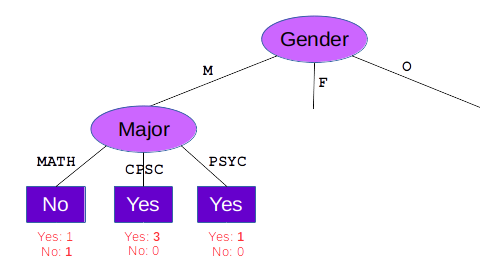
\includegraphics[width=0.7\textwidth]{maleMajorSplit.png}
\caption{The tree-in-progress if we choose to split on \textsf{Major} in the
male branch.}
\label{fig:maleMajorSplit}
\end{figure}

\begin{samepage}
Our other choice, of course, is to split on \textsf{Age} instead:

\begin{Verbatim}[fontsize=\footnotesize,samepage=true,frame=single,framesep=3mm]
students[students.Gender=="M"].groupby('Age').VG.value_counts()
\end{Verbatim}
\vspace{-.2in}
\end{samepage}

\begin{Verbatim}[fontsize=\small,samepage=true,frame=leftline,framesep=5mm,framerule=1mm]
Age     VG 
middle  No     1
        Yes    1
old     Yes    1
young   Yes    3
Name: VG, dtype: int64
\end{Verbatim}

Again, 5 out of 6 correct. Here, \texttt{middle}-aged students are the only
heterogeneous group; the \texttt{old} folks and \texttt{young}-uns are clean
splits. With this choice, our tree would appear as in
Figure~\ref{fig:maleAgeSplit}.

\begin{figure}[ht]
\centering
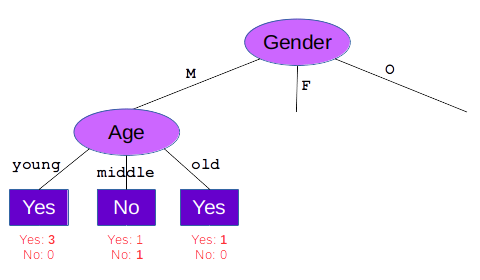
\includegraphics[width=0.7\textwidth]{maleAgeSplit.png}
\caption{On the other hand, the tree-in-progress if we choose to split on
\textsf{Age} in the male branch instead.}
\label{fig:maleAgeSplit}
\end{figure}

So at this point, since splitting on either feature and then stopping would
give us exactly 5 out of 6 points correct, we just flip a coin. I just flipped
one, and it came out tails (for \textsf{Age}) -- hope that's okay with you.

\subsubsection{Finishing up the left branch}

The two ``Yes'' leaves in Figure~\ref{fig:maleAgeSplit} are now set in stone,
since every single \texttt{young} male in our training set was indeed a
videogamer, as was every \texttt{old} male. Now we just have to deal with the
\texttt{middle} branch.

Only one feature now remains to split on -- \textsf{Major} -- so we'll do that,
and produce the result in Figure~\ref{fig:maleAgeMiddle}. There's exactly one
\texttt{middle}-aged male \texttt{MATH} major in the original
\texttt{DataFrame} (line 12, p.~\pageref{vgDataSet}), and he's labeled ``No,''
so we'll guess ``No'' in the \texttt{MATH} branch. Similarly, we have one data
point to guide us for \texttt{CPSC} majors (line 3), so we'll predict ``Yes''
in this case. The \texttt{PSYC} branch presents a conundrum, though: our data
set doesn't have \textit{any} \texttt{middle}-aged male Psychology majors, so
how do we know what to guess in this case?

\begin{figure}[ht]
\centering
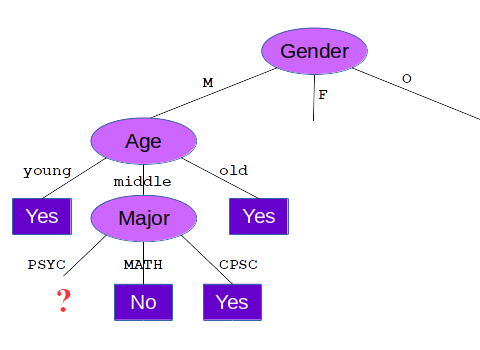
\includegraphics[width=0.8\textwidth]{maleAgeMiddle.png}
\caption{Going one level further down after splitting on \textsf{Age} for
males. We have data for \texttt{middle}-aged \texttt{CPSC} and \texttt{MATH}
males...but what to do with \texttt{middle}-aged \texttt{PSYC} males?}
\label{fig:maleAgeMiddle}
\end{figure}

The best way to handle this is to fall back to a more general case where you
\textit{do} have examples. It's true that we have no training points for
\texttt{middle}-aged male Psychology majors, but we \textit{do} have points for
\texttt{middle}-aged males-in-general, and we discovered that 5 out of 6 of
them were gamers. So it makes sense to default to ``Yes'' in the \texttt{PSYC}
branch of this part of the tree, even though we don't have any data points
exactly like that. So that's what we'll do. The finished left branch is
depicted in Figure~\ref{fig:maleAgeMiddleWithPsyc}.

\begin{figure}[ht]
\centering
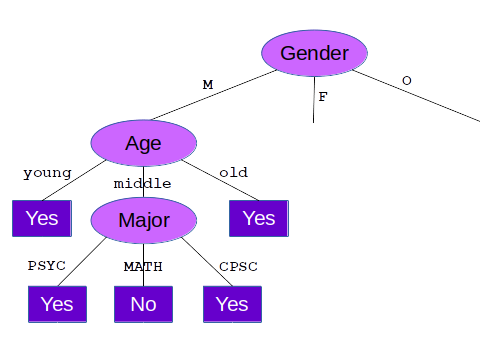
\includegraphics[width=0.7\textwidth]{maleAgeMiddleWithPsyc.png}
\caption{The decision tree we're in the process of inducing, with the left
branch entirely completed.}
\label{fig:maleAgeMiddleWithPsyc}
\end{figure}

\subsubsection{Finishing up the rest of the tree}

The rest of the process is just the same stuff done over and over.\footnote{If
you're wondering whether there's a way to automate this, the answer is a
resounding \textbf{yes}! There are many packages in Python and other languages
which will automatically build a decision tree from a training set; the
\texttt{DecisionTreeClassifier} from the \texttt{scikit-learn} package is one
of them. This exercise of learning how to build a decision tree manually is so
you can understand the concepts of what's going on under the hood -- kind of
like you learn how to add numbers in grade school even though you'll normally
use a calculator later on in life.} At each branch of the tree, we take the
subset of the training points that remain (\textit{i.e.}, the training points
that match the path from the root thus far, and are therefore applicable), and
decide what to branch on next. When we get to a completely homogeneous group,
we stop and put a leaf there. The end result of all these efforts is the final
decision tree for the videogame data set, in Figure~\ref{fig:completeVgTree},
and its Python equivalent in Figure~\ref{fig:completeVgTreePython}.

\index{contradiction (in a training set)}

One interesting aspect of our final tree is the
female$\rightarrow$\texttt{PSYC}$\rightarrow$\texttt{middle}-aged branch.
You'll see that this leaf is labeled ``Yes(?)'' in the diagram. Why the
question mark? Because this is the one case where we have a
\textbf{contradiction} in our training data. Check out lines 2 and 16 back on
p.~\pageref{vgDataSet}. They each reflect a \texttt{middle}-aged female
Psychology major, but with \textit{different} labels: the first one is not a
videogame player, but the second one is.

I always thought the term ``contradiction'' was amusing here. Two similar
people don't have exactly the same hobbies -- so what? Is that really so
surprising? Do all middle-aged female Psychology majors have to be identical?

Of course not. But you can also see things from the decision tree's point of
view. The \textit{only} things it knows about people are those three
attributes, and so as far as the decision tree is concerned, the people on
lines 2 and 16 really \textit{are} indistinguishable. When contradictions
occur, we have no choice but to fall back on some sort of majority-rules
strategy: if out of seven otherwise-identical people, two play videogames and
five do not, we'd predict ``No'' in that branch. In the present case, we can't
even do \textit{that} much, because we have exactly one of each. So I'll just
flip a coin again. (\texttt{*flip*}) It came up heads, so we'll go with
``Yes.''

Notice that in this situation, the resulting tree will actually misclassify one
or more \textit{training} points. If we called our function in
Figure~\ref{fig:completeVgTreePython} and passed it our person from line 2
(\texttt{\textquotesingle PSYC\textquotesingle}, \texttt{\textquotesingle
middle\textquotesingle}, \texttt{\textquotesingle F\textquotesingle}), it would
return \texttt{"Yes"} even though line 2 is not a gamer. Furthermore,
contradictions are the \textit{only} situation in which this will ever happen;
if the data is contradiction-free, then every training point will be classified
correctly by the decision tree.

Paradoxically, it turns out that's not necessarily a good thing, as we'll
discover in Volume II of this series. For now, though, we'll simply declare
victory.

\begin{figure}[ht]
\centering
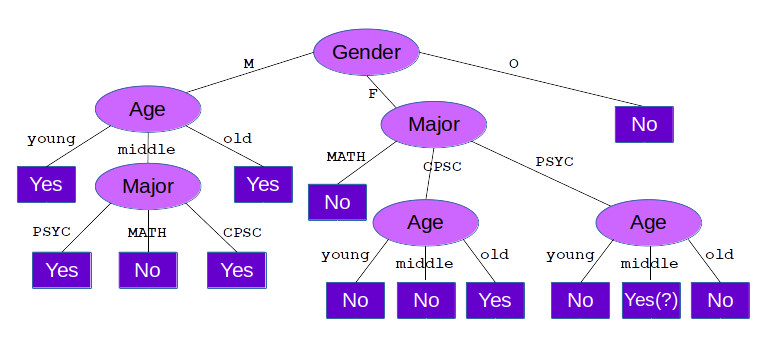
\includegraphics[width=1\textwidth]{completeVgTree.png}
\caption{The final decision tree for the videogame data set.}
\label{fig:completeVgTree}
\end{figure}

\begin{figure}[ht]
\centering
\begin{Verbatim}[fontsize=\footnotesize,samepage=true,frame=single,framesep=3mm,xleftmargin=.2cm,xrightmargin=.2cm]
def predict(major, age, gender):
    if gender == 'M':
        if age == 'young':
            return 'Yes'
        elif age == 'middle':
            if major == 'PSYC' or major == 'CPSC':
                return 'Yes'
            elif major == 'MATH':
                return 'No'
        elif age == 'old':
            return 'Yes'
    elif gender == 'F':
        if major == 'MATH':
            return 'No'
        elif major == 'CPSC':
            if age == 'young' or age == 'middle':
                return 'No'
            elif age == 'old':
                return 'Yes'
        elif major == 'PSYC':
            if age == 'young' or age == 'old':
                return 'No'
            elif age == 'middle':
                return 'Yes'  # Here's our "contradiction"
    elif gender == 'O':
        return 'No'
\end{Verbatim}
\caption{The final decision tree for the videogame data set, as a Python
function.}
\label{fig:completeVgTreePython}
\end{figure}

% split a numerical attribute into categorical
